\chapter{XMPP: Extensible Messaging and Presence Protocol}
\label{chap:XMPP}

At the start of 1999, an open instant messaging protocol was released by Miller
under the name Jabber \cite{XSF-History}, along with a server implementation,
\textit{jabberd}. Unlike the various commercial instant messaging protocols
provided by America On-Line (AOL) \cite{AIM}, Microsoft \cite{MSN} and Yahoo
\cite{Yahoo} that required reverse engineering to create third-party clients,
Jabber was an open specification based on streaming Extensible Markup Language
(XML).

In the following year, the Internet Engineering Task Force (IETF) finished work
on both a model and requirements for an \textit{Internet Messaging and Presence
Protocol} (IMPP) \cite{RFC2778}\cite{RFC2779}; no implementation was produced
by the working group, and in 2002 the Jabber community had organized enough
to submit the Jabber protocol as a proposed implementation for IMPP, but with
the name changed to the \textit{Extensible Messaging and Presence Protocol}
\cite{RFC3920}\cite{RFC3921}. In early 2004, the XMPP specifications were
formalized and approved by the IETF as Proposed Standards \cite{XSF-History}.
The protocol continues to be updated and expanded by the XMPP Standards
Foundation (XSF).

\section{The XMPP Network}
\label{sec:The-XMPP-Network}

XMPP defines two wire-format protocols to enable server to client and server to
server communications. The result is a decentralized client-server architecture,
similar in structure to the one used for email with the \textit{Simple Mail
Transfer Protocol} (SMTP). Each server maintains long-lived connections
to many clients, and optionally connections to other XMPP servers. For
the most popular server implementation, \texttt{ejabberd} \cite{ejabberd}
\cite{XSF-Services}, accepting upwards of twenty-thousand clients on a regular
basis is possible \cite{JabberRu}, particularly when implementation specific
clustering is used to spread server loads across multiple physical machines
\cite{ejabberd-cluster}. Figure \ref{fig:Jabber.ru-Statistics} shows a snapshot
of the daily usage of the the Russian Jabber.ru XMPP server, which processes
approximately fourteen thousand client connections at any given time. Other
large XMPP installations, notably Google's GTalk \cite{GTalk} and Facebook's
chat \cite{Facebook} services, are able to accept, through clustering, several
million clients at once.

\begin{figure}
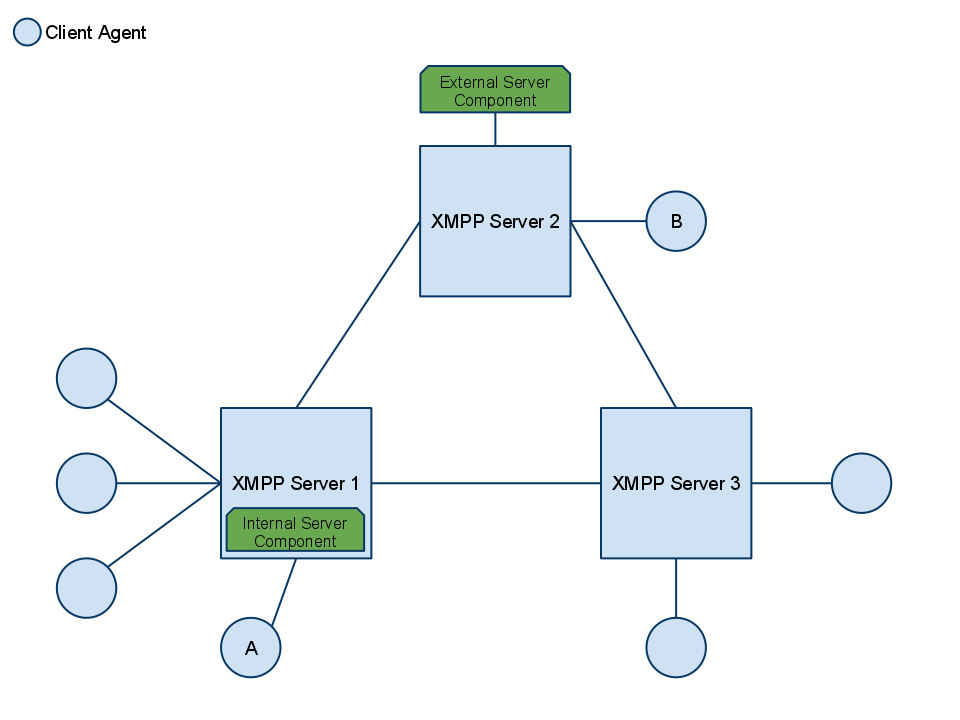
\includegraphics[width=\columnwidth]{figures/xmpp_network}
\label{fig:XMPP-Network}
\caption{A demonstration of a basic XMPP network, including client agents,
internal and external server components, and XMPP servers. Communications
from entities associated with one server are not routed by any intermediary
server. Messages sent from the client marked ``A'' to the client marked ``B''
will always be sent from server labeled ``1'' to the server labeled ``2'',
never along the path from ``1'' to ``3'' to ``2''.}
\end{figure}

\begin{figure}
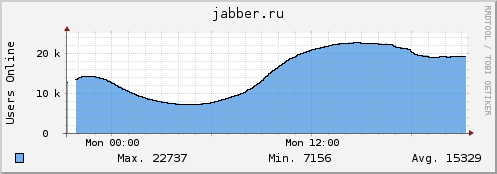
\includegraphics[width=\columnwidth]{figures/jabber_ru_stats}
\label{fig:Jabber.ru-Statistics}
\caption{Daily usage graph from the Russian XMPP service provider Jabber.ru.
Average use is around 22,000 simultaneous client connections during peek 
daytime hours.}
\end{figure}

While many server implementations provide the ability to cluster, XMPP itself
does not define a clustering mechanism. Instead, it provides a mechanism for
separate server installations to \textit{federate}, allowing communications
between clients hosted by either server. Unlike the federation allowed by
SMTP, XMPP mandates at most two servers will process any message between two
clients; in SMTP, the number of intermediate servers in unbounded. The limit on
intermediate servers is aimed at limiting message spoofing and other types of
spam common in the SMTP network. Figure \ref{fig:XMPP-Network} shows the 
various configurations an XMPP network may take.

\section{Jabber IDentifiers (JIDs)}
\label{sec:JIDs}

Each entity within an XMPP network is addressable using one or more
\textit{Jabber Identifiers}, or JIDs \cite{RFC3920}. The JID used by any
connected entity is globally unique, based on the Domain Name System (DNS).
JIDs commonly look similar to e-mail addresses, but with an additional section:
\texttt{localpart@domainpart/resourcepart}. The \texttt{<domainpart>} portion
of the JID is the only required section. JIDs for servers consist solely
of the domain name exposing the XMPP service (DNS service, or SRV, records
can be used to allow a server to support a domain different from the domain
of the machine on which it is running \cite{RFC3920}). User accounts on a
server are identified by the \texttt{<localpart>} section of the JID; when
only the form \texttt{localpart@domainpart} is used, the result is called
a \textit{bare JID}. When a client connects to a server using an account's
bare JID, then the connection is assigned a resource value to distinguish
it from any other connections already established by that user account;
a JID with all three sections is referred to as a \textit{full JID}, and
it is the full JID that is globally unique. To demonstrate, if a client
connects to the \texttt{kestrel.cs.clemson.edu} server using the bare JID
\texttt{user@kestrel.cs.clemson.edu}, then the particular connection established
may be assigned the full JID \texttt{user@kestrel.cs.clemson.edu/133742}.

\section{Types of XMPP Agents}
\label{sec:Types-of-XMPP-Agents}

Within the network are four types of entities, or agents, which can be marked
on a continuum of scalability. The first is the regular XMPP client; many
implementations for clients exist, notably for use with instant messaging by a
human. However, many client agents exist as automated programs, or \textit{bots}
\cite{RFC3921}, to provide services to other clients in the network. Each
client connection is associated with a unique full JID (server implementations
are free to decide to reject duplicate full JIDs connections or terminate the
existing connection in favor of the new one \cite{RFC3920}). Under
the XMPP Design Guidelines, clients are typically kept simple, offloading as
much functionality as possible onto the server, making it easier for multiple
implementations to work together \cite{XEP-0134}.

The next step up in terms of scalability is the external server component.
XMPP acknowledges that servers will not always provide built-in support
for all desired features; thus, servers may be easily extended through
components. External components are separate programs, possibly running on a
different machine than the server, that are trusted by the server. A standard
wire-protocol is used between servers and components, making external components
interroperable with any server implementation.Each component is assigned a
subdomain from domain used by the server, and all JIDs using that subdomain
are forward by the server with no additional processing to the component;
it is left to the component how to interpret the JIDs provided to it. For
example, a multi-user chat component will treat the username portion of a JID
as the chat room name, and the resource as a participant's nickname within
the room, i.e. for the component \texttt{conference.jabber.org}, the JID
\texttt{sleek@conference.jabber.org/Lance} would refer to the participant named
``Lance'' within the ``sleek'' chat room on the \texttt{jabber.org} server.

The greater scalability afforded by a component is due to the server's lack
of responsibility for the JIDs used by the component. For a normal client,
the server is tasked with maintaining a roster of subscriptions between the
client and other entities in the network. For human centered clients, this
relationship works well due to typically small roster sizes for which the
server is optimized. As roster sizes increase, two scalability issues emerge.
The first is that the optimization assumption of small rosters is violated,
potentially impacting performance based on the storage mechanisms used. The
second is that a client's roster is sent to the client in a single stanza as
part of the initialization procedure of the XMPP session. Stanzas are not
interruptible -- all other stream communications to the client are blocked while
the roster is transmitted \cite{Moffitt2008a}. For rosters with several
thousand entries, this places a severe penalty on start up times for agents and
on the amount of networking traffic used \cite{Moffitt2008}. For a
component, no roster is maintained by the server, leaving that responsibility to
the component itself.

The final two entity types are internal server components and servers themselves.
Internal server components receive the same benefits as external components, but
they are implemented in a server-dependent fashion. Their main advantage is the
ability to hook directly into the server's internals to provide services that
would not be as easily done otherwise. The final tier of potential scalability
is to create a custom implementation that speaks the server to server protocol,
eliminating the need for many features provided by traditional servers.

\section{Stanzas}
\label{sec:Stanzas}

Communications between an XMPP client and server are done using two streams of
XML data, one for each direction of communication. Each stream starts with the
\texttt{<stream:stream xmlns="etherx.jabber.org/streams" />} element, and all
\textit{stanzas} sent or received during the session will be top-level children
of one of these two elements. At the conclusion of an XMPP session, the stream
elements are terminated, creating two valid XML documents \cite{RFC3920}. The
sections of XML transmitted during the session are not full XML documents,
and as such are referred to as stanzas instead. Each stanza is guaranteed to
possess certain attributes, namely the attributes \texttt{to} and \texttt{from}
which provide the JIDs identifying the sender and recipient of the stanza
\cite{RFC3920}. In general, the \texttt{from} attribute of a stanza is set by
the server in order to combat impersonation \cite{RFC3920}. While
there are several elements that may appear at the top-level of a stream element
during the course of establishing the session, there are three main elements
that are defined to be stanzas: \texttt{<message />}, \texttt{<presence />},
and \texttt{<iq />}. Each type of stanza differs in both routing and response
behaviors.

\subsection{Message}
\label{sec:Message}

The most basic of the three stanza types, a \texttt{<message />} stanza is used
to push data from one agent to another. While this is typically done in a ``fire
and forget'' manner, some servers support more advanced message processing that
can provide better guarantees of message delivery \cite{XEP-0079}. However, even
with reliable delivery, there is no guaranteed response from a \texttt{<message
/>} stanza. The most common use for \texttt{<message />} stanzas is as an
envelope for messages from a chat session between two agents. Other major uses
include broadcasting event notices from a publish-subscribe mechanism.

\subsection{Presence}
\label{sec:Presence}

The \texttt{<presence />} stanza is used to multicast data, namely presence
and status information, to other agents that have subscribed for it. Each
\texttt{presence} stanza may include a status message, a value indicating the
current state of the agent (such as free for chat, away, do not disturb, etc),
and a priority value indicating the relative importance of the connection
amongst other connections from the same bare JID. Some servers use the priority
value when routing stanzas by sending stanzas addressed to the bare JID
to the resource with the highest priority value. While it is possible to
include additional information in a \texttt{<presence />} stanza, it is highly
discouraged. Presence stanzas are typically the most frequently stanzas used
within an XMPP network, and thus bandwidth usage must be considered and
minimized \cite{RFC3921}.

Presence stanzas whose \texttt{type} attribute value is in one of
\texttt{subscribe}, \texttt{subscribed}, \texttt{unsubscribe}, or
\texttt{unsubscribed} are used to create and remove presence subscriptions,
and thus the roster. Subscriptions are directional, and it is not required
to establish mutual subscriptions. When a presence stanza is sent to the
server without a JID for particular recipient, the server will broadcast
the stanza to all connected agents that have subscribed to the particular
agent's presence. The process for establishing a subscription is done by
first sending a \texttt{<presence />} stanza possessing a \texttt{type} value
of \texttt{subscribe}, or \texttt{<presence type="subscribe" />}. If the
receiving entity approves the request, it will respond with a \texttt{<presence
type="subscribed" />} stanza. The receiving entity may then choose to repeat
the process in reverse to subscribe to the initial agent's presence. If the
entity refuses the request, a \texttt{<presence type="unsubscribed" />} stanza
is issued instead. Ending a subscription is done by sending a \texttt{<presence
type="unsubscribe" />} stanza to an entity. The receiving agent will then
respond with a \texttt{<presence type="unsubscribed" />} stanza.


\subsection{Info/Query (IQ)}
\label{sec:Iq}

The final stanza is the \texttt{<iq />} stanza, which is short for
``Info/Query''. In contrast with \texttt{<message /} stanzas, \texttt{<iq
/>} stanzas are guaranteed to have a response, either from another agent, or
the server itself. There are four types of \texttt{<iq /} stanzas, two for
requests and two for responses. An initial \texttt{<iq />} request may possess a
\texttt{type} value of either \texttt{get} or \texttt{set}. A \texttt{get} type
is roughly equivalent to the HTTP \texttt{GET} method. These requests are meant
to request some form of data from another agent, usually without other side
effects. A \texttt{set} type corresponds to the HTTP \texttt{POST} method, and
is used to send information to another agent, with the usual intention for it to
be saved or perform some side effect.

When an \texttt{<iq />} is successfully processed, a response \texttt{<iq />}
with a \texttt{type} value of \texttt{result} will be returned. A response
with a \texttt{type} value of \texttt{error} indicates that an error occurred
somewhere during the exchange, such as the intended recipient was not found or
the recipient could not handle the request. It is possible to associate the
initial \texttt{<iq />} stanza with its response by examining its \texttt{id}
attribute. Every stanza used by XMPP includes an \texttt{id} attribute, and that
value is used as the \texttt{id} value of a reply stanza.

\section{Security Considerations}
\label{sec:Security-Considerations}

In order to provide basic security to XMPP communications between clients
and servers, the Transport Layer Security (TLS) \cite{TLS} and Simple Authentication
and Security Layer (SASL) \cite{SASL} must be used. The use of TLS provides
channel encryption for the XML stream to prevent tampering and eavesdropping \cite{RFC3920}.
While it is a requirement to support the use of TLS in both client and server 
implementations, it is still possible for a server administrator to make its
use optional. Client agents requiring a secure channel must negotiate the use
of TLS using the STARTLS \cite{RFC3920} stream feature. The method of encryption
used by TLS is commonly based on digital certificates, which must be validated
by a client agent when presented to ensure a valid chain-of-trust for the
server's certificate; this may be done either by explicitly comparing the presented
certificate against a known, trusted version, or checking that the certificate
has been issued by a trusted Certificate Authority (CA).

While TLS prevents tampering, it does not guarantee the identity of the client
initiating the communications. SASL provides several mechanisms for allowing
a client to authenticate an identity. These mechanisms include:
\begin{enumerate}
\item PLAIN: The client's password is transmitted in base64 encoding, relying
on the underlying stream's channel encryption for security.
\item DIGEST-MD5: A more secure form of authentication whereby the client is
challenged by the server to provide a hashed version of the user's password,
along with the username, server name, security realm, etc \cite{RFC2831}. The
main advantage is that the password itself is never transmitted.
\item EXTERNAL: The SASL EXTERNAL mechanism allows for a client to authenticate
itself using a digital certificate.
\end{enumerate}

While each connection between entities in the XMPP network may be encrypted,
the core XMPP standards do not define a method for end-to-end encryption of
data. Several methods for achieving end-to-end encryption have been proposed,
but a consensus has not yet been reached. An older method is documented 
in XEP-0027: Current Jabber OpenPGP Usage \cite{XEP-0027} whereby message or
presence stanza contents may be encrypted using an OpenPGP key. Unfortunately,
IQ stanza contents can not be encrypted in this manner. A newer proposal
uses IQ stanzas to implement a secondary communications channel, whose contents
is encrypted using TLS \cite{XMPP-E2E}.

\section{XMPP Extension Proposals (XEPs)}
\label{sec:XEPs}

While the core XMPP specifications are maintained by the IETF, the XMPP
Standards Foundation is responsible for maintaining additional extensions to
the specifications and protocols, adding new features or documenting current
best practices. Such extensions are referred to as XMPP Extension Proposals,
or XEPs, each of which is assigned a four digit number starting from 0001.
XEPs are grouped into several categories, including \textit{Draft Standard},
\textit{Final Standard}, \textit{Experimental}, \textit{Deferred}, among
others \cite{XEP-0001}. A XEP in the final standard state is considered
finished, and will not be updated further. A draft standard XEP is considered
stable and reliable for implementation, while an experimental XEP is encouraged
for implementation but may still undergo significant revision. Several XEPs are
considered fundamental to providing robust and useful XMPP services.

\subsection{Service Discovery: XEP-0030}
\label{sec:Service-Discovery}

It is useful and necessary for an entity within an XMPP network to query other
entities about their identities, supported features, and any related entities
within the network. For this purpose, XEP-0030 Service Discovery \cite{XEP-0030}
defines the use of ``disco'', short for service discovery, using \texttt{<iq />}
stanzas. Disco is broken into two categories: information and items. The information
portion is used to query and report identities and feature support. The items portion
is used to return a list of JIDs related to an agent.

An important concept introduced by XEP-0030 is the idea of a ``node'' for a JID. A node
refers to an aspect, or facet of the services provided by a JID \cite{XEP-0030}. For
example, an agent may provide two distinct services. By specifying a node, the disco
query can be limited to only requesting information about one particular service.

An identity in XMPP is a combination of a \texttt{category}, \texttt{type}, \texttt{name}, and
\texttt{lang}. The category and type values are selected from a predefined set that is used
to identify the agent as a human facing client, or a server component providing a gateway
service to another instant messaging network. Features are specified by listing the 
recognized namespaces used by the supported features.

An agent may also be responsible, or be the authoritative reference, for other JIDs used
in the network. One such case would be a multi-user chat component's responsibility for
JIDs for the chat rooms it provides. Each JID provided in the query results may also 
include a node name to refer to particular services or information resources provided
by a single JID.

\subsection{Entity Capabilities: XEP-0115}
\label{sec:Entity-Capabilities}

While service discovery provides a useful and generic mechanism for querying
for features supported by other entities, the bandwidth required to perform
to walk through the various nodes provided by a JID to build a complete disco
profile can be considerable when working with many agents. XEP 0115, Entity
Capabilities, allows for simplifying the disco process by including a hashed
version of a node's identities and features in a \texttt{<presence />} stanza.
When an agent receives such a presence notice, it will query the sender to
retrieve the full contents matching the given hash value, provided that the
hash value is one that has not been seen before. Under the assumption that many
agents will have identical sets of identities and features, due to using the
same underlying client libraries, the issue of excess bandwidth consumption is
minimized.

\subsection{Data Forms: XEP-0004}
\label{sec:Data-Forms}


\subsection{Ad-hoc Commands: XEP-0050}.
\label{sec:Adhoc-Commands}


